\chapter{Theoretical Underpinning}
\label{cha:theory}


In this chapter, the predominant theories defining the approach adopted by the Tiles toolkit and the IoT ideation process will be presented. It is worth mentioning that the investigation work that led to the creation and evaluation of the Tiles toolkit and the IoT ideation process was grounded in additional theories such as UCD, end-user development (EUD), SCL and CSRL and took advantage of the HCI guidelines, for example, in connection to usability. Some of these theoretical domains have been addressed in Chapter~\ref{cha:smart-cities}, whereas others will be covered in Chapter~\ref{cha:research-methodology}.


\section{Co-Design}

In the context of sustainable HCI, distinctions were drawn between seeing the behaviour of the users as the cause of environmental problems and gathering needs and opportunities from users to inform design \autocite{disalvo_mapping_2010}. By means of participation and co-design, people can provide direct input to \textit{solve the problem of the users}, designing thus their own behaviour change \autocite{lockton_designing_2014}.
Through co-design, users build empathy with the solution they contributed to. Co-design allows multiple voices to be heard; it is fair and ethical to involve those whose livelihoods, environments and lives are at stake in the decisions that affect them \autocite{perlgut_community_2005}.
Employing participatory approaches empowers people, allowing shared responsibilities among stakeholders. This can create credibility and trust, emphasise diversity in stakeholder involvement and increase the likelihood that the final product will meet the expectations \autocite{pettersen_ethics_2008}. The role of the researchers is to support, explain, fight and help negotiate design tensions, recommending methods and tools. Controlling the creative process and managing the users are practices that do not belong to the co-design methodology.

Under the umbrella of co-design, various approaches and methods are used, which result in different combinations between the level of involvement of the stakeholders and the number of different stages of the design process covered. Many studies that apply co-design in the smart city context involve the users during the brainstorming and idea generation phase \autocites{mitchell_empirical_2016}{schuurman_smart_2012}{mechant_e--deliberation_2012}{fu_building_2014}, whereas others consider the shareholders only in a tokenistic way, limiting their contribution to the act of providing simple feedback or rating the final solution \autocite{reiersolmoen_delta_2017}.
Although participation is historically emphasised at the moment of idea generation \autocite{cross_design_1971}, modern co-design practices can extend beyond the very first phases of the design process, including the users more deeply throughout the whole process. This is facilitated by the lower entry barriers achievable while using recent technologies to address specific tasks, which have been a prerogative of professionals only a few years ago.

In this thesis, I will describe how co-design practices have been used to drive brainstorming and idea generation and also how co-design can be extended beyond its traditional scope. This aspect characterises how the toolkits described in Chapter~\ref{cha:iot-framework} are intended to be used \textit{in the wild}. The objective is to promote a co-design process where potential stakeholders are brainstorming, designing and prototyping a solution for a problem that affects them.
This opportunity has been explored in few studies, which is demanding given the social and technological challenges that come attached to practices like design validation with the user and collaborative implementation of ideas.


\section{Tangible User Interaction with Smart Objects}

The work described in this thesis embraces the understanding of IoT and ubiquitous computing proposed by Rogers \autocite*{rogers_moving_2006}, which challenges the original calm computing vision of Weiser \autocite*{weiser_computer_1991}. Weiser depicted a scenario where user interaction is anticipated and predicted by a sensing smart environment, relegating the user to a mostly passive role.
This approach led to poor results in research and prototyping on ubiquitous computing and IoT, mainly because trying to predict human will is a difficult artificial intelligence problem \autocite{rogers_moving_2006}. Even small errors are perceived as annoying and frustrating from the user, to the point of dismissing and abandoning the technology in use.

Such vision presents challenges also from a sociological point of view. Users should be encouraged to interact and make critical decisions; the technology can support this process, improving awareness, stimulating reflection and possibly engaging the user in the activity.
This way, it is possible to introduce new techniques to change the attitudes and behaviours of people, on the basis of social learning, for sustainable common objectives.

Rogers did not completely discard the vision of Weiser but rather tried to entertain other possibilities besides calmness for research on ubiquitous computing.
Examples include extending and supporting personal, cognitive and social processes such as habit-changing, problem-solving, creating, analysing, learning or performing a skill \autocite{rogers_moving_2006}.
Rogers advocated that research in the field should be aimed at better understanding human activity rather than trying to predict and intervene in situations that already work reasonably well, with a high risk of unwanted or unpredictable outcomes. This people-oriented perspective was also envisioned by Streitz et al. \autocite*{streitz_designing_2005} in the smart object research domain. They prospected smart objects as empowering artefacts for decision-making, supporting mature and responsible actions.

In order to tackle the challenges described in Section~\ref{sec:motivation}, I chose to adopt an \textit{object augmentation} strategy in order to create TUIs based on smart objects. As described by Kuniavsky \autocite*[p. 254]{kuniavsky_smart_2010}, object augmentation starts from everyday, non-digital objects and augments them with technology, while their purpose and familiar characteristics are maintained.
This family of interfaces, also called sensing-based interfaces, allows for new interaction paradigms that explore the opportunities lying beyond traditional human-computer interfaces such as screens, keyboards and mice \autocite{van_dam_post-wimp_1997}. TUIs are characterised by the embodiment of interaction in physical objects, they emphasise the physicality of interaction through the coupling of physical and digital representations \autocite{markova_tangible_2012}.
TUIs take advantage of the physical skills of the users, exploiting knowledge of the everyday, non-digital objects \autocite{jacob_reality-based_2008}.
These physical interfaces are capable of delivering relevant information at appropriate times, which is critical for triggering learning and sustaining reflection \autocite{rogers_framework_2006}. In addition, they can be embedded into the environment and represent data streams in a physical way \autocite{hornecker_getting_2006}. User interaction then moves \textit{off the screen}, becomes more natural and can be distributed in space \autocite{dourish_where_2004}.

\begin{figure}[hbt]
    \centering 
	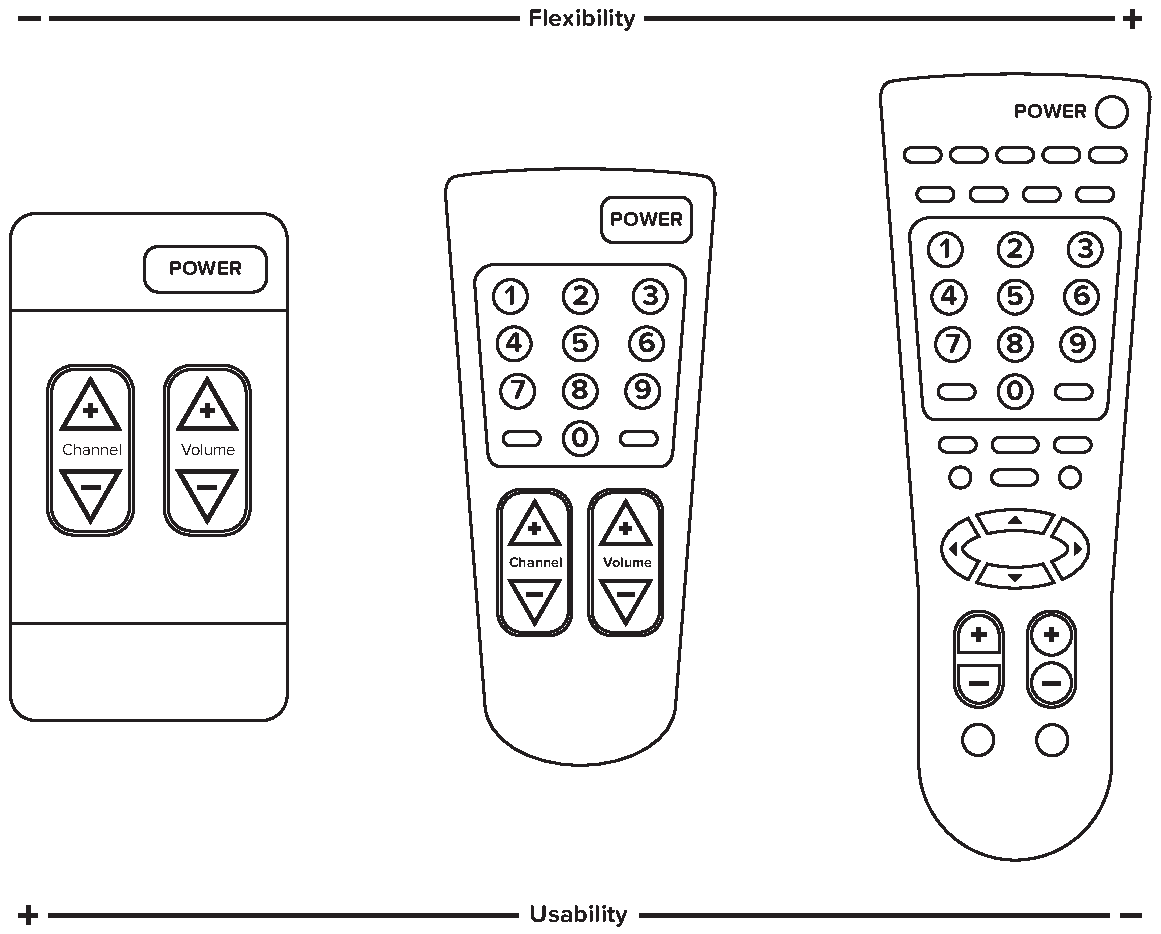
\includegraphics[width=\textwidth]{remotes}
	\caption{A visual example of how a simple design can be easy to use, whereas a more flexible and feature-rich one is less usable \autocite[p. 103]{lidwell_universal_2010}.}
	\label{fig:remotes}
\end{figure}

Advocating the well-known design maxim \textit{\enquote{jack of all trades, master of none}}, Lindwell et al. \autocite*[p. 102]{lidwell_universal_2010} presented the trade-off between \textit{flexibility} and \textit{usability} in design: flexible designs can perform more functions than specialised ones do, but they perform these functions less efficiently (Fig.~\ref{fig:remotes}). Jacob \autocite*{jacob_reality-based_2008} transferred this concept to TUIs, proposing a trade-off between \textit{reality} and \textit{versatility}. TUIs are specialised by their physical affordances and constraints and, thus, can perform a limited set of tasks with a high level of realism or simplicity. Moreover, TUIs foster collaboration \autocite{rogers_configuring_2003}, in which they increase the visibility of the actions of others and allow for concurrent interactions. TUIs extend the static representation of an object with an intangible, dynamic one. TUIs were part of the original vision of Weiser and have been then researched by Rogers as well as Ullmer and Ishii \autocite*{ullmer_emerging_2000}, among others.


